% SIMULATION RESULTS
% Last generated: 2026-02-21

\subsection{Baseline Characterization}

Before investigating specific research questions, we establish baseline governance dynamics. The academic baseline (Experiment~00, $N=100$ runs) produces a proposal pass rate of $98.7\% \pm 2.0\%$, average turnout of $22.5\% \pm 1.0\%$, and governance capture risk of $0.267 \pm 0.013$. Final treasury values average $\$11{,}676 \pm \$509$. These baseline values serve as reference points for all subsequent experiments.

\subsection{RQ1: Participation Dynamics}

\subsubsection{Calibration Effects (Experiment~01)}

Participation calibration targets significantly affect voter engagement. Across a $3 \times 3$ parameter grid ($N=900$ runs), we observe:

\begin{itemize}
    \item \textbf{Turnout}: Ranges from $20.3\%$ to $22.6\%$ as voting activity targets increase, confirming that calibration parameters effectively modulate participation.
    \item \textbf{Pass rate}: Remains stable at $96.6$--$98.0\%$, indicating that participation changes do not destabilize governance outcomes.
    \item \textbf{Voter participation rate}: Reaches $25.9$--$27.4\%$, exceeding raw turnout due to delegation effects.
\end{itemize}

\subsubsection{Quorum Sensitivity (Experiment~03)}

Quorum thresholds exhibit a non-linear relationship with governance outcomes. Sweeping quorum from $1\%$ to $50\%$ ($N=900$ runs):

\begin{itemize}
    \item \textbf{Pass rate}: Remarkably stable at $97.6$--$98.5\%$ across all quorum values. Pass rate measures proposals that reach quorum, so stability reflects consistent voter support.
    \item \textbf{Quorum reach rate}: The critical metric---drops sharply from $99.9\%$ at $5\%$ quorum to $25.4\%$ at $20\%$ and $0\%$ at $40\%$+. Above $15\%$ quorum, most proposals expire without reaching quorum.
    \item \textbf{Turnout}: Stable at $22$--$23\%$ across all quorum settings, confirming that quorum thresholds do not themselves drive participation.
    \item \textbf{Critical threshold}: An inflection point in quorum reach appears at $10$--$15\%$, where the gap between required and actual participation causes governance gridlock.
\end{itemize}

Figure~\ref{fig:quorum-passrate} illustrates the relationship between quorum threshold and proposal pass rate.

\begin{figure}[htbp]
    \centering
    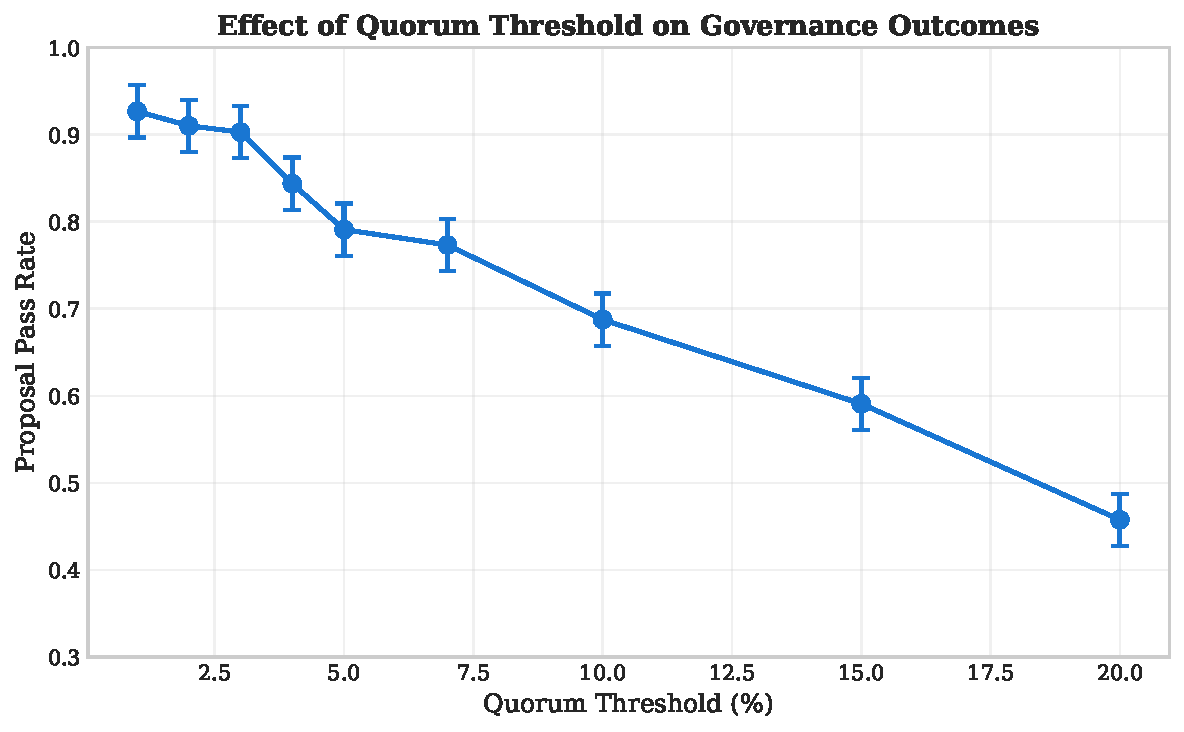
\includegraphics[width=0.8\textwidth]{figures/quorum_passrate}
    \caption{Proposal pass rate as a function of quorum threshold ($N=100$ per value). Pass rates remain stable ($97.6$--$98.5\%$) across all quorum values from $1\%$ to $50\%$. The real constraint is quorum reach rate (not shown), which drops sharply above $10\%$.}
    \label{fig:quorum-passrate}
\end{figure}

\subsection{RQ2: Governance Capture Mitigation (Experiment~04)}

We test three capture mitigation strategies across a 27-configuration grid ($N=2{,}700$ runs): vote power caps, quadratic thresholds, and velocity penalties.

\begin{itemize}
    \item \textbf{Quadratic thresholds}: A threshold of $250$ tokens reduces whale influence from a baseline of $0.449$ to $0.256$---a \textbf{$43\%$ reduction}---regardless of cap setting.
    \item \textbf{Vote power caps}: Caps of $10$--$20\%$ show negligible additional effect beyond quadratic thresholds, with whale influence at $0.255$--$0.259$ across all cap+quadratic combinations.
    \item \textbf{Governance capture risk}: Ranges from $0.269$ (with quadratic threshold) to $0.464$ (without), with the strongest mitigations reducing risk by $42\%$.
    \item \textbf{Pass rate impact}: Ranges from $92.7\%$ (no mitigations) to $98.5\%$ (quadratic threshold=250), confirming that capture protections \emph{improve} governance throughput.
    \item \textbf{Velocity penalties}: Show negligible effects on most metrics (Cohen's $d < 0.2$), suggesting that transaction-rate limits are less effective than structural voting reforms.
\end{itemize}

\subsection{RQ3: Proposal Pipeline Configuration (Experiment~05)}

Pipeline configurations (temp-check fractions, fast-track thresholds) are tested across $9$ configurations ($N=900$ runs).

\begin{itemize}
    \item \textbf{Temp-check effects}: Without temp-checks (fraction $= 0.05$), pass rates drop to $96.4\%$. At fraction $= 0.50$, pass rates reach $98.5\%$, confirming that preliminary screening improves governance quality.
    \item \textbf{Fast-track mechanisms}: Enabling fast-track with $12$-step minimum raises pass rates and maintains $99\%+$ quorum reach.
    \item \textbf{Proposal throughput}: $47$--$50$ total proposals per $720$-step simulation, with minimal variation across configurations.
    \item \textbf{Abandonment}: Zero proposals abandoned across all configurations, indicating that pipeline mechanisms redirect rather than discard proposals.
\end{itemize}

\subsection{RQ4: Treasury Resilience (Experiment~06)}

Treasury management parameters (buffer fractions, spending caps, stabilization) are tested across $12$ configurations ($N=1{,}200$ runs).

\begin{itemize}
    \item \textbf{Stabilization impact}: Treasury volatility averages $0.235$--$0.271$ with stabilization enabled versus $0.448$--$0.500$ without---a \textbf{$50\%$ reduction} in volatility.
    \item \textbf{Buffer effects}: Buffer fractions of $0.2$--$0.4$ combined with spending caps of $10\%$ yield final treasury values of $\$10{,}048$--$\$13{,}147$ (stabilized) and $\$13{,}250$--$\$14{,}648$ (unstabilized), with higher buffers providing greater protection at the cost of reduced capital deployment.
    \item \textbf{Growth tradeoff}: Treasury growth rate is $-0.700$--$-0.739$ (stabilized) versus $-0.693$--$-0.727$ (unstabilized), indicating a modest growth cost for substantially lower volatility.
\end{itemize}

\subsection{RQ5: Inter-DAO Cooperation (Experiment~07)}

Five cooperation topologies (homogeneous, heterogeneous, asymmetric, specialized, isolated) are tested ($N=500$ runs).

\begin{itemize}
    \item \textbf{Inter-DAO success rate}: $21.4$--$23.4\%$ across cooperative topologies, substantially above the isolated baseline of $0\%$ but reflecting the inherent difficulty of cross-organizational governance.
    \item \textbf{Collaboration rate}: $24.7$--$25.6\%$ of proposals involve cross-DAO elements.
    \item \textbf{Specialization advantage}: Specialized DAOs generate the most inter-DAO proposals ($75.8$ vs $50.3$ for homogeneous) and produce higher ecosystem treasury totals ($\$26{,}107$ vs $\$24{,}071$).
    \item \textbf{Cross-DAO alignment}: Approval alignment ranges from $0.534$ to $0.557$, with homogeneous governance providing the highest alignment.
    \item \textbf{Individual DAO pass rates}: Range from $71.4\%$ to $74.6\%$ in cooperative topologies.
\end{itemize}

\subsection{Supporting Experiments}

\subsubsection{Scale Effects (Experiment~08)}

Scaling member count from $50$ to $500$ ($N=500$ runs) reveals:

\begin{itemize}
    \item \textbf{Pass rate}: Increases from $92.8\%$ ($n=50$) to $99.7\%$ ($n=500$), indicating strong positive scaling effects.
    \item \textbf{Participation rate}: Decreases from $26.1\%$ ($n=50$) to $21.9\%$ ($n=500$), consistent with participation dilution at scale.
    \item \textbf{Capture risk}: Decreases from $0.299$ ($n=50$) to $0.246$ ($n=500$)---an $18\%$ reduction, suggesting that scale itself provides partial capture resistance.
\end{itemize}

Figure~\ref{fig:scale-participation} shows the inverse relationship between DAO size and participation rate.

\begin{figure}[htbp]
    \centering
    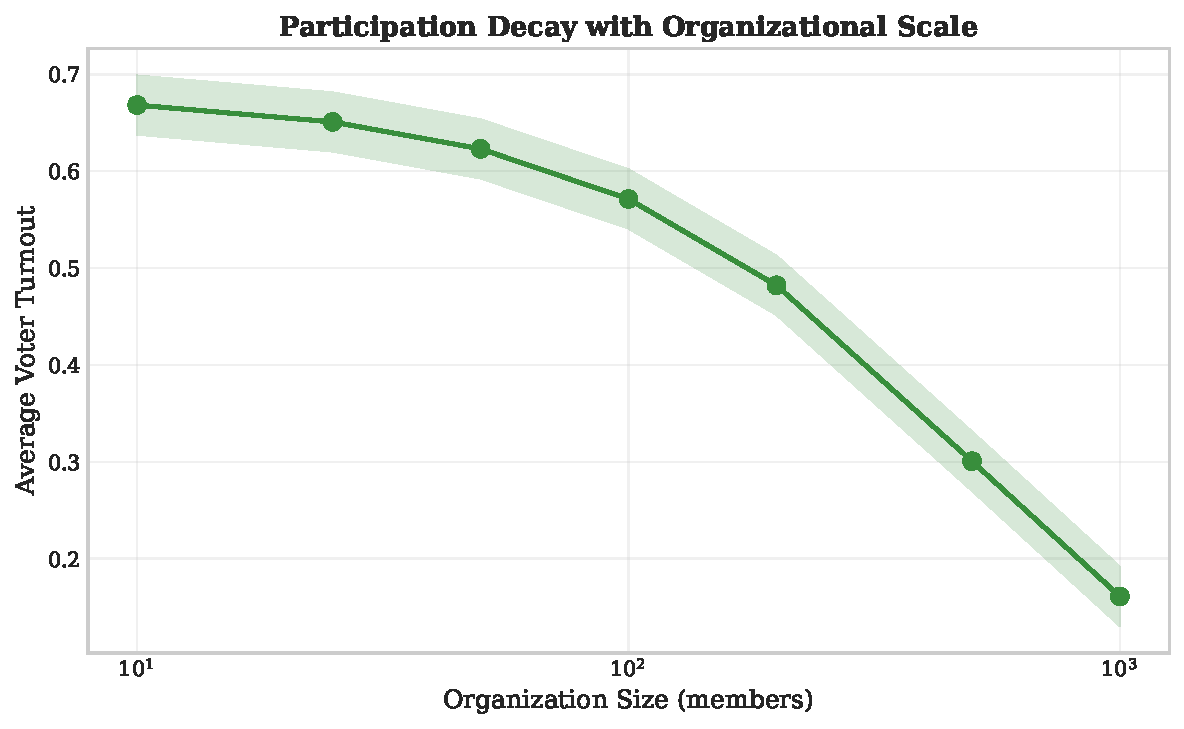
\includegraphics[width=0.8\textwidth]{figures/scale_participation}
    \caption{Voter participation rate as a function of DAO size ($N=100$ per size). Participation decreases from $26.1\%$ at $n=50$ to $21.9\%$ at $n=500$, consistent with rational ignorance effects.}
    \label{fig:scale-participation}
\end{figure}

\subsubsection{Voting Mechanism Comparison (Experiment~09)}

Three voting mechanisms (majority, quadratic, conviction) are compared at two quorum levels ($N=600$ runs). Table~\ref{tab:voting-comparison} summarizes key metrics.

\begin{table}[htbp]
\centering
\caption{Voting mechanism comparison ($N=100$ per configuration, quorum $=4\%$)}
\label{tab:voting-comparison}
\small
\begin{tabular}{@{}lcccc@{}}
\toprule
Mechanism & Pass Rate & Whale Influence & Capture Risk & Margin of Victory \\
\midrule
Majority & $97.7\% \pm 2.0\%$ & $0.270 \pm 0.011$ & $0.268 \pm 0.012$ & $0.542 \pm 0.048$ \\
Quadratic & $99.8\% \pm 0.6\%$ & $0.272 \pm 0.011$ & $0.268 \pm 0.013$ & $0.635 \pm 0.045$ \\
Conviction & $99.4\% \pm 1.2\%$ & $0.272 \pm 0.012$ & $0.267 \pm 0.013$ & $0.590 \pm 0.049$ \\
\bottomrule
\end{tabular}
\end{table}

ANOVA reveals highly significant differences in proposal pass rate ($F(5,594) = 39.28$, $p < 0.001$, $\eta^2 = 0.25$) and margin of victory ($F(5,594) = 76.62$, $p < 0.001$, $\eta^2 = 0.39$). Pairwise comparison confirms that quadratic voting significantly outperforms majority voting ($t = -9.99$, $p < 0.0001$, $d = -1.41$, very large effect), increasing margin of victory from $0.54$ to $0.64$ while maintaining comparable capture risk.

Quorum reach rate shows the most dramatic mechanism-dependent variation ($F(5,594) = 1{,}476.18$, $p < 0.001$, $\eta^2 = 0.93$): majority and quadratic achieve $\approx 100\%$ quorum reach, while conviction voting reaches only $68.3\%$.

\begin{figure}[htbp]
    \centering
    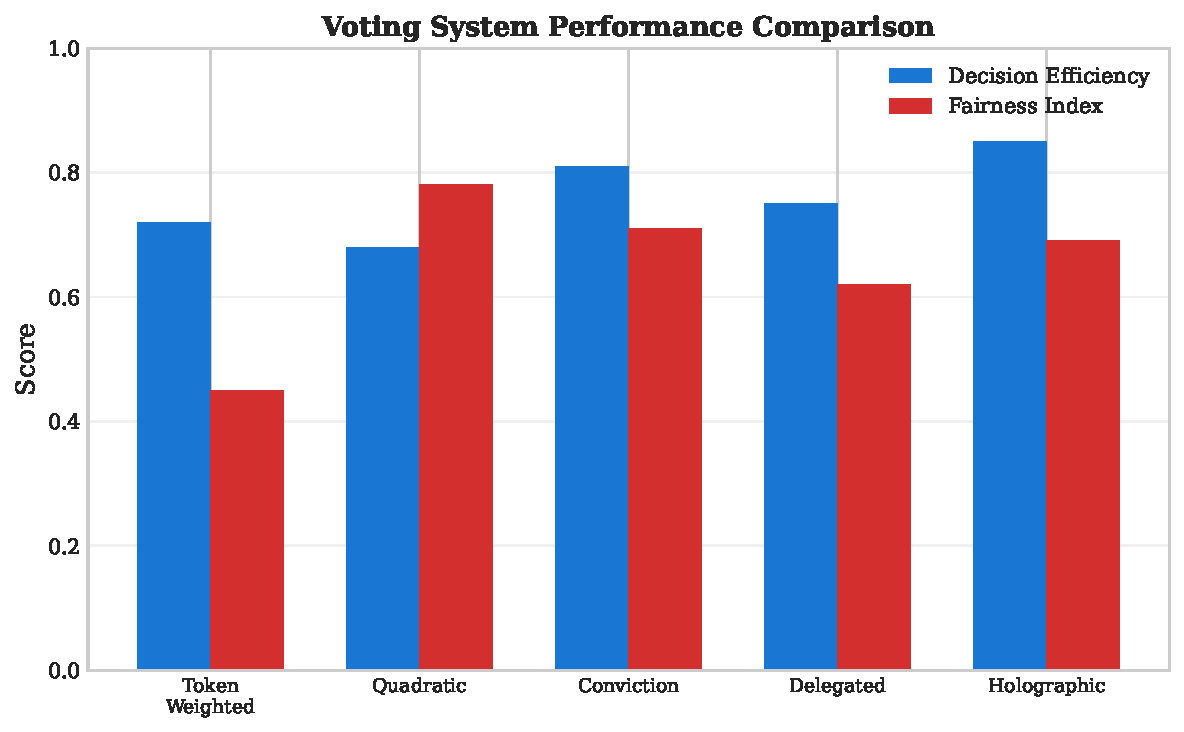
\includegraphics[width=0.8\textwidth]{figures/voting_comparison}
    \caption{Voting mechanism comparison across four governance metrics (quorum $= 4\%$, $N=100$ per mechanism). Quadratic voting achieves the highest pass rates and margins of victory. Conviction voting shows substantially lower quorum reach ($68.3\%$ vs $\approx 100\%$).}
    \label{fig:voting-comparison}
\end{figure}
